% !TEX program = pdflatex
% Traitement du signal, vincent.mazet@unistra.fr

\documentclass[11pt, twoside, a4paper]{article}

% Packages généraux
\usepackage[T1]{fontenc}
\usepackage[utf8]{inputenc}
\usepackage{amsfonts, amsmath, amssymb}
\usepackage{microtype}

% Graphiques
\usepackage{graphicx}
\usepackage{tikz}

% Typo française
\usepackage[french]{babel}
\frenchspacing
\DecimalMathComma

% Mise en page
\usepackage{enumitem}
\usepackage{multicol}
\usepackage[margin=2cm]{geometry}
\sloppy
\parindent 0mm

% Métadonnées du PDF
\usepackage[
  pdftitle={Traitement du signal},
  pdfauthor={Vincent MAZET (Université de Strasbourg)},
  breaklinks=true,
  pdfborder={0 0 .5}]{hyperref}

% Exercice (sans coefficient, avec titre)
\newcounter{exercise}[section]
\newcommand{\exo}[1]{%
  \refstepcounter{exercise}%
  \subsubsection*{Exercice~\theexercise\ifstrempty{#1}{}{~: #1}}
}

\begin{document}

  \makebox[3cm][l]{FIP ESN 1\textsuperscript{re} année} \hfill Traitement du signal \hfill \makebox[3cm][r]{2023--2024}
  \begin{center}
    \LARGE\textbf{Classification des signaux}
  \end{center}
\bigskip\bigskip

% ==================================================================================================================== %

Placez dans les onze éléments ci-dessous dans les cercles gris du tableau.

\bigskip

\begin{multicols}{3}
\begin{enumerate}[label= \raisebox{.5pt}{\Large\textcircled{\raisebox{-.5pt}{\normalsize\arabic*}} } ]
  \item signal quantifié
  \item signal échantillonné
  \item signal analogique
  \item signal numérique
  \item numérisation
  \item échantillonnage
  \item quantification
  \item \raisebox{-11mm}{\includegraphics[width=30mm]{signal-analogique}}
  \item \raisebox{-11mm}{\includegraphics[width=30mm]{signal-echantillonne}}
  \item \raisebox{-11mm}{\includegraphics[width=30mm]{signal-numerique}}
  \item \raisebox{-11mm}{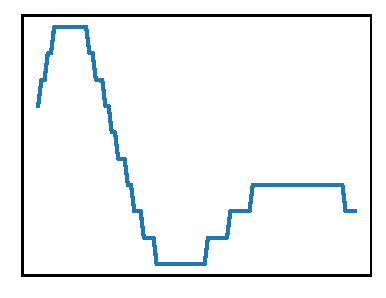
\includegraphics[width=30mm]{signal-quantifie}}
\end{enumerate}
\end{multicols}

\bigskip\bigskip

\begin{center}
  \begin{tikzpicture}
    % Cadre
    \draw (0,-2) -- (15,-2) -- (15,-15) -- (0,-15) -- (0,-2) ;
    % Lignes horizontales
    \draw (0,-5) -- (15,-5) ;
    \draw (0,-10) -- (15,-10) ;
    % Lignes verticales
    \draw (5,-2) -- (5,-15) ;
    \draw (10,-2) -- (10,-15) ;
    % Ligne diagonale
    \draw (0,-2) -- (5,-5) ;
    % Textes
    \draw (4.5,-2.5) node[below left]{Temps} ;
    \draw (0.5,-4.5) node[above right]{Amplitude} ;
    \draw ( 7.5,-3.5) node {\parbox{30mm}{\centering Signal à\\temps continu}} ;
    \draw (12.5,-3.0) node {\parbox{30mm}{\centering Signal à\\temps discret}} ;
    \draw (2.5, -7.5) node {\parbox{30mm}{\centering Signal à\\valeurs continues}} ;
    \draw (2.5,-12)   node {\parbox{30mm}{\centering Signal à\\valeurs discrètes}} ;
    % Cercles échantillonné/quantifié
    \draw [thick, fill=black!10] (2.5,-13.25) circle (.5) ;
    \draw [thick, fill=black!10] (12.5,-4.0)  circle (.5) ;
    % Cercles dans les cases
    \draw [thick, fill=black!10] (6.8,-7.5)   circle (.5) ;
    \draw [thick, fill=black!10] (8.2,-7.5) circle (.5) ;
    \draw [thick, fill=black!10] (12.5, -7.5) circle (.5) ;
    \draw [thick, fill=black!10] (11.8,-12.5) circle (.5) ;
    \draw [thick, fill=black!10] (13.2,-12.5) circle (.5) ;
    \draw [thick, fill=black!10] ( 7.5,-12.5) circle (.5) ;
    % Cercles en dehors des cases
    \draw [<-, >=latex, thick] (11,-11) arc (0:90:2);
    \draw [thick, fill=black!10] (10.4,-9.6) circle (.5) ;
    \draw [<-,>=latex, thick] (11.35,-2.4) arc (45:135:2);
    \draw [thick, fill=black!10] (10,-1.8) circle (.5) ;
    \draw [->,>=latex, thick] (.4,-8.65) arc (135:225:2);
    \draw [thick, fill=black!10] (-.2,-10) circle (.5) ;
  \end{tikzpicture}
\end{center}

% ==================================================================================================================== %

\end{document}
